\chapter{Lecture 24 - Solving Systems of 1\textsuperscript{st}-Order IVPs}
\label{ch:lec24n}
\section{Objectives}
The objectives of this lecture are to:
\begin{itemize}
\item Apply Euler's explicit method to solve systems of 1\textsuperscript{st}-order IVPs
\item Show how to convert higher order IVPs into systems of 1\textsuperscript{st}-order IVPs
\end{itemize}
\setcounter{lstannotation}{0}

\section{Systems of 1\textsuperscript{st}-Order IVPs with Euler's Explicit Method}
So far we have only addressed scalar first-order equations.  There are many physical phenomena that, in order to properly describe the relevant physics, must be modeled as a system of equations.  In this section we will consider the dynamics of the isotope xenon-135 in nuclear reactors.

\subsection{Xenon-135 Background}

Most nuclear reactors in the world today generate power through the fission of $^{235}\text{U}$.  Each fission results in the release of approximately 185 MeV of recoverable energy,\sidenote{MeV stands for ``mega-electron-volt'', or $1\times 10^6$ eV.  1eV is equivalent to $1.6 \times 10^{-19}$ Joules. It takes a lot of fissions to produce a discernable amount of power.} two or three neutrons, one or more of which is expected to also cause a fission thus propagating the chain reaction, and two fission products.  Almost all of the resulting fission products are radioactive, needing to undergo a series of beta- and alpha-decay processes to achieve a nuclear configuration that is stable.  This process is depicted in Figure \ref{fig:FissionProductDecayChain}.
\begin{marginfigure}
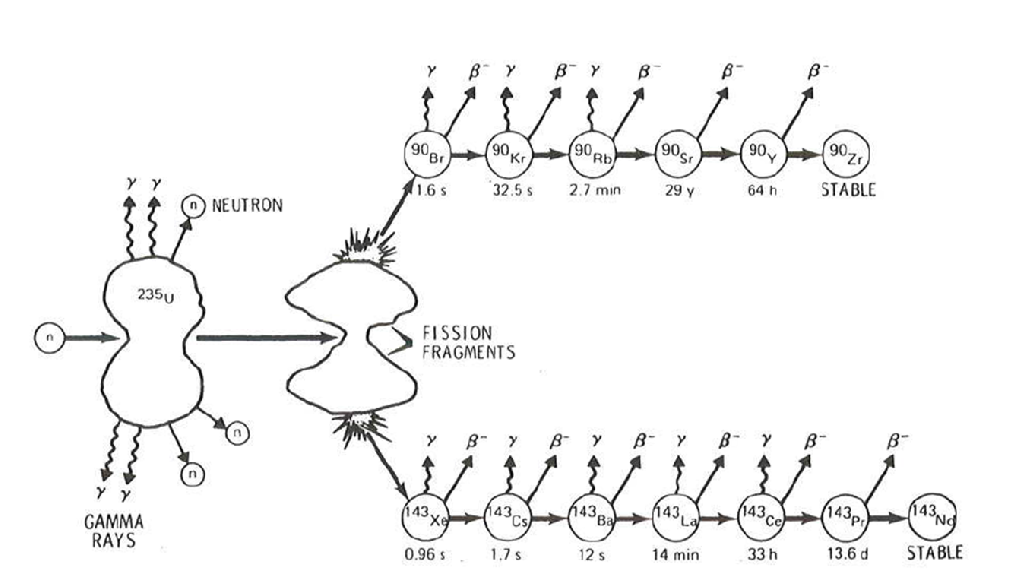
\includegraphics{FissionProductDecayChain.eps}
\caption{Schematic of representative fission product decay process.}
\label{fig:FissionProductDecayChain}
\end{marginfigure}

Some of these fission products (and their subsequent decay offspring) have a significant impact on the nuclear chain reaction that goes on around them.  One class of fission products very influential in this way are those that have a strong tendency to absorb neutrons without undergoing fission.  These fission products are sometimes referred to as \emph{poisons}, owing to the fact that neutron absorption ``poisons'' the chain reaction process by preventing the absorbed neutron from going on to cause fission of an atom of fuel.


The particular fission product decay chain that produces $^{135}$Xe is illustrated in Figure \ref{fig:decayChain}.  Tellurium-135 $\left(^{135}\text{Te}\right)$ is produced directly from fission.  It undergoes beta-decay to iodine-135 $\left(^{135}\text{I}\right)$ with a 19-second half-life.  $^{135}\text{I}$ in turn decays to xenon-135 $\left(^{135}\text{Xe}\right)$ with a slower half-life of 6.6 hours. $^{135}\text{Xe}$ is also produced in significant quantities as a fission product. $^{135}\text{Xe}$ undergoes both beta-decay to cesium-135 $\left(^{135}\text{Cs}\right)$ as well as neutron absorption---denoted with the $(n,\gamma)$ symbol for radiative capture---to become $^{136}\text{Xe}$ which is stable but a very weak neutron absorber.  $^{135}\text{Cs}$ decays to barium-135 $\left(^{135}\text{Ba}\right)$ which is a strong neutron absorber, but since the half-life is 2.3 million years, not enough $^{135}\text{Ba}$ builds up in the core to have an impact on the kinetic behavior of the fission process.
\begin{marginfigure}[-4.0cm]
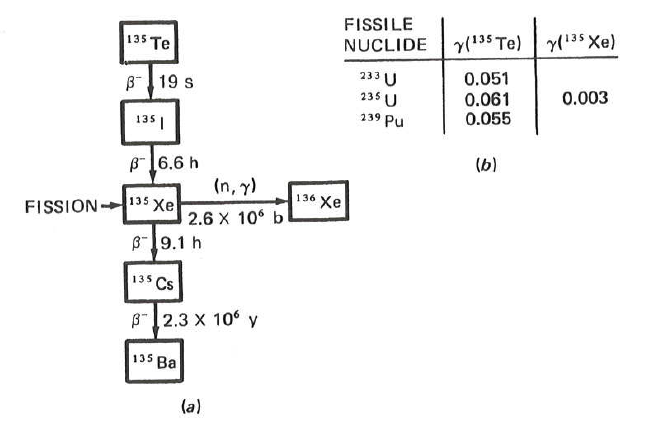
\includegraphics{decayChain.png}
\caption{Fission product decay chain for generating xenon-135.}
\label{fig:decayChain}
\end{marginfigure}

\subsection{Model of $^{135}$Xe Concentration}
We can model the atom density of $^{135}$I and $^{135}$Xe with a first-order system of differential equations.
\marginnote{Owing to the short halflife of $^{135}$Te we assume that it immediately decays and thus, effectively, is a direct production term for $^{135}$I.

\vspace{0.15cm}

\noindent Nomenclature:
\begin{enumerate}
\item I - iodine-135 atom density
\item Xe - xenon-135 atom density
\item $\phi$ - neutron flux.  Flux is proportional to reactor power; if flux is higher, reactor power is higher.
\item $\gamma$ - fission yield. The fraction of fissions that result in a particular fission product.
\item $\lambda$ - decay constant which is related to half-life: $\lambda = \sfrac{\ln{(2)}}{\text{t}_{\sfrac{1}{2}}}$
\item $\sigma_{a}$ - microscopic absorption cross-section. Represents the probability that an incident neutron will be absorbed.  Neutron ``poisons'' have large values of $\sigma_a$.
\end{enumerate}
}
\begin{align*}
\frac{d\text{I}}{dt} &= \overbrace{\gamma^{\text{Te}}\Sigma_f \phi}^{\substack{\text{production from}\\\text{fission}}} -\overbrace{\lambda^{\text{I}}\text{I}}^{\substack{\text{loss from}\\\text{decay}}}\\
\frac{d\text{Xe}}{dt} &= \underbrace{\gamma^{\text{Xe}}\Sigma_f\phi}_{\substack{\text{production}\\ \text{from}\\\text{fission}}} + \underbrace{\lambda^{\text{I}}\text{I}}_{\substack{\text{production}\\\text{from iodine}\\\text{decay}}} - \underbrace{\lambda^{\text{Xe}}\text{Xe}}_{\substack{\text{loss from}\\\text{xenon}\\\text{decay}}} - \underbrace{\text{Xe}\sigma_a \phi}_{\substack{\text{loss from}\\\text{neutron}\\\text{capture}}}
\end{align*}
This system can be solved using Euler's explicit method more-or-less in the same way that a single equation can be solved with the following equations:
\begin{align*}
y(t) &= \bracketVectorstack{\text{I(t)} \\ \text{Xe(t)}} \\
y^{\prime}(t) &= \bracketVectorstack{\text{I}(t) \\ \text{Xe}(t)}^{\prime} = \bracketVectorstack{\gamma^{\text{Te}} \Sigma_f \phi - \lambda^{\text{I}}y(1,t) \\ \gamma^{\text{Xe}}\Sigma_f \phi + \lambda^{\text{I}}y(1,t) - \lambda^{\text{Xe}}y(2,t)-y(2,t)\sigma_a \phi} 
\end{align*}
and the time-stepping formula would be:\marginnote[0.5cm]{\textbf{Note:} Here we adopt the MATLAB syntax for vectors.  We also use $dt$ to indicate the step-size.}
\begin{equation*}
y(:,t+1) = y(:,t) + y^{\prime}(:,t) \text{dt}
\end{equation*}

\subsection{MATLAB Implementation}

An analysis of $^{135}$Xe concentration through a typical power transient comprising a reactor start-up, a period of full power during which xenon levels approach equilibrium, and then a brief shutdown followed by a start-up 20 hours later is shown in the next few listings. 

\vspace{0.5cm}

\noindent We start by clearning the environment and providing necessary nuclear data. \marginnote{

\vspace{2.5cm} 

\noindent\ref{lst:ann24n-1} We us a local function (defined below) to specify the time-dependent flux profile for the transient of interest.

}
\begin{lstlisting}[style=myMatlab,name=lec24n-ex1]
clear
clc
close 'all'

%% Nuclear Data
nominalFlux = 2e14; % n/cm^2-s  
flux = @(t) nominalFlux*power_profile_Xe(t); /*!\annotation{lst:ann24n-1}!*/
Sigma_F = .0452; %1/cm 
% Iodine-135  and Tellurium-135 Nuclear data
gamma_Te = 0.061; 
lambda_I = 2.9173e-5; %1/s

% Xenon-135 Nuclear data
sigma_a_Xe = 2.6e6*10^(-24); % cm^2
gamma_Xe = 0.003; 
lambda_Xe = 2.1185e-5; % 1/s 
\end{lstlisting}
\noindent Next we will set time intervals for the explicit Euler method and initialize data arrays.
\begin{lstlisting}[style=myMatlab,name=lec24n-ex1]
%% Time discretization
tStart = 0; % sec - time start
tEnd = 160*3600; %sec -  time end (160 hours)
numTs = 50000; 
tSpace = linspace(tStart,tEnd,numTs);
dT = tSpace(2)-tSpace(1);

%% Construct data arrays and provide initial conditions
P = nan(2,numTs+1); % an extra column for the initial data
P(1,1) = 0; % initial I-135 concentration;
P(2,1) = 0; % initial Xe-135 concentration;
pfrac = nan(1,numTs); % power fraction

\end{lstlisting}
\noindent Now we are ready to commence time stepping.\marginnote{

\vspace{1.0cm}

\noindent\ref{lst:ann24n-2} For scripts that require more than a few seconds to run, it is a good practice to provide some intermediate output to let the user know that ``something is happening.''  At the same time, you also do not want to flood the command window with output.  Here we choose to provide a progress update every 10000 time steps.  

\vspace{0.25cm}

\noindent\ref{lst:ann24n-3} The notation here is somewhat clunky but these lines effectively define $y^{\prime}$.
}
\begin{lstlisting}[style=myMatlab,name=lec24n-ex1]
%% Commence time stepping
for ts = 1:numTs      

    if mod(ts,10000)==0  /*!\annotation{lst:ann24n-2}!*/
        fprintf('Commencing time step %i.\n',ts);
    end       
     
    dP = nan(2,1);
    T = tSpace(ts);
    pfrac(ts) = power_profile_Xe(T);
    % update Iodine concentration
    dP(1) = gamma_Te*Sigma_F*flux(T) - lambda_I*P(1,ts);  /*!\annotation{lst:ann24n-3}!*/
    % update Xenon concentration
    dP(2) = gamma_Xe*Sigma_F*flux(T) + lambda_I*P(1,ts) ...
        - P(2,ts)*sigma_a_Xe*flux(T) - lambda_Xe*P(2,ts);  
          
    % update the total poison concentration.
    P(:,ts+1) = P(:,ts) + dP*dT;    
end
\end{lstlisting}

\noindent Once the calculations are done, we will plot the results.  For this transient analysis the output is shown in Figure \ref{fig:lec24n-xenon-transient-plot}.
\begin{marginfigure}[2.5cm]
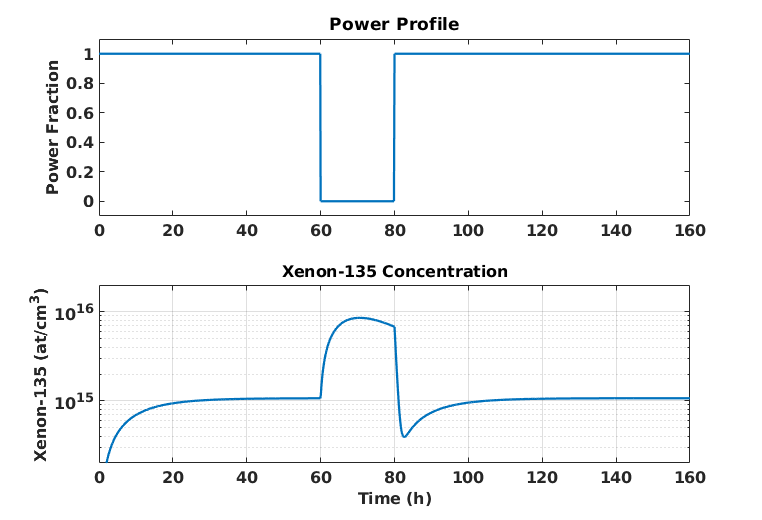
\includegraphics{lec24n-xenon-transient-plot.png}
\caption{Xenon-135 concentration during a transient.}
\label{fig:lec24n-xenon-transient-plot}
\end{marginfigure}
\begin{lstlisting}[style=myMatlab,name=lec24n-ex1]
%% Plot your results
figure(1)
subplot(2,1,1)
plot(tSpace/3600,pfrac,'linewidth',2);
axis([0 160 -0.1 1.1]);
title('Power Profile')
set(gca,'fontsize',14,'fontweight','bold');
ylabel('Power Fraction',...
    'FontWeight','bold','FontSize',14);

subplot(2,1,2)
h = semilogy(tSpace/3600,P(2,1:(end-1)));
set(h,'linewidth',2);
set(gca,'fontsize',14,'fontweight','bold');
axis([0 160 2*10^14 2*10^16])
grid on
xlabel('Time (h)','FontWeight','bold','FontSize',14)
ylabel('Xenon-135 (at/cm^3)',...
    'FontWeight','bold','FontSize',14);
title('Xenon-135 Concentration','FontSize',14,...
    'FontWeight','bold')
\end{lstlisting}
The power profile for the transient is encoded in a local function as shown below.
\begin{lstlisting}[style=myMatlab,name=lec24n-ex1]
%% Local Functions
function p = power_profile_Xe(t)
% returns a power level [0,1] giving the percent full power
tH = t/3600; % convert seconds to hours.
if tH < 60
    p = 1;
elseif tH>=60 && tH<80
    p = 0;
else
    p = 1;
end
end
\end{lstlisting}

\section{Convert High-Order IVPs into a System of 1\textsuperscript{st}-Order IVPs}
Now that we have introduced a few methods for numerically solving initial value problems, some readers may be starting to wonder when we will include methods taylored to solve IVPs of 2\textsuperscript{nd}-, 3\textsuperscript{rd}-, or 4\textsuperscript{th}-order.  The (possibly) surprising answer is that we will \emph{not} present new methods for solving higher-order IVPs.  Instead, \emph{all} of the numerical methods we present for IVPs will be for 1\textsuperscript{st}-order IVPs; higher-order IVPs will simply be re-stated in terms of a system of 1\textsuperscript{st}-order IVPs.
